%%%%%%%%%%%%%%%%%%%%%%%%%%%%%%%%%%%%%%%%%%%%%%
%                insertmeeting
% 1) Title (something creative & funny?)
% 2) Date (MM/DD/YYYY)
% 3) Location (ex. Hagerty High School)
% 4) People/Committees Present 
% 5) Picture 
% 6) Start Time & Stop Time (ex. 12:30AM to 4:30PM)
%%%%%%%%%%%%%%%%%%%%%%%%%%%%%%%%%%%%%%%%%%%%%%
\insertmeeting 
	{Daring Designs} 
	{11/26/21}
	{Hagerty High School}
	{James, Nathan, Ritam}
	{Images/RobotPics/robot.jpg}
	{1:30 - 4:30}
	
\hhscommittee{Hardware}
\noindent\hfil\rule{\textwidth}{.4pt}\hfil
\subsubsection*{Goals}
\begin{itemize}
    \item Decide material for side plates
    \item Design more rigid side plates to support the arm
  

\end{itemize} 

\noindent\hfil\rule{\textwidth}{.4pt}\hfil

\subsubsection*{Accomplishments}
Because we are switching our intake focus from a new design back to fixing up the old one for now, the cad committee wants to also pivot to another project, that like the new intake won’t be ready for the upcoming meet, but will be implemented later on in the season. Doing the CAD now not only will give us another project to work on, but will take stress away from us in the future by getting ahead of the game. The problem that we are trying to solve is one that our driver noticed while driving at meet 1. The rev extrusions we used to support the arm, although functional, are slightly flexible which makes the arm harder to make small adjustments to. The way we want to fix this is by replacing the rev extrusions with a custom made piece that will extend farther backwards, giving more support to the arm. We also plan to use these new side plates to display our numbers and protect our electronics, replacing the corrugated plastic sides that currently serve those purposes.
Thinking of designs, we started thinking of materials and making sketches for what the side plates would look like (Figure \ref{fig:pic1}). Seeing the success of the front bumper, we started with the idea of making the sides out of folded sheet metal which is strong, not too heavy, and able to be custom designed. Going into onshape, we used our newly learned skills with the sheet metal tools to create a prototype of the sideplates (Figure \ref{fig:pic2}). While working on this design, we noticed a crucial problem with using sheet metal, which was that we can only put a flange facing one direction, which will mean that where the metal sheet bends to connect to the drivetrain will be mostly unsupported. This undermines the entire point of redesign, as it may make the sides unstable. Although there may be a way to make the sheet metal work, we talked to one of our mentors, Mr. Harper, about alternate design ideas. One idea he brought up that we thought sounded very interesting was making the sides out of carbon fiber. There is a way to create custom carbon fiber pieces using a mold that we can design and 3d print and a vacuum pump. Because we can 3d print a mold, we can make the sides almost whatever shape we need with very few limitations. Carbon fiber also has the advantage of being both stronger and lighter than aluminum. 
After deciding to go with the carbon fiber option, we made some basic sketches and talked to our mentor about what the best shape for the sides would be. Because the mold will be 3d printed, the sides can be almost whatever shape we decide, leading us to the decision to make the sides a smooth wave-like shape that moves inwards as it goes up (Figure \ref{fig:pic3}). We plan to leave the bottom of the sides wider apart to give space for the REV hubs and wiring, also allow the space to be open enough for us to fix or change the wiring if needed. 
Moving into onshape, we worked backwards, first creating what we wanted the sides to look like, planning to make the mold after the sides were  complete.  We started creating the left side, initially thinking that we could just mirror it for the right side, but we soon realized that we had not left enough space for the REV core hex motor that pivots the arm.  Because we still wanted the general shape to remain the same, we decided to make the right side slightly different by making the curve steeper, allowing space for the motor to attach inside the plates.  After finishing the left side (Figure \ref{fig:pic4}) we moved on to the right side.  Although we wanted part of it to be steeper to hold the motor, most of the right side would be identical to the left.  Because of this, we were able to create a mirror of the left side for a portion of the right side. To create the remaining part of the right side, we created a new sketch with a steeper slope, as we had planned (Figure \ref{fig:pic5}). We blended the two sections together using onshape’s loft tool, which kept the side (Figure \ref{fig:pic6}).  With that step complete, all that is left is to create the molds, which we plan to do at a future meeting.

 

\begin{figure}[ht]
\centering
\begin{minipage}[b]{.48\textwidth}
  \centering
  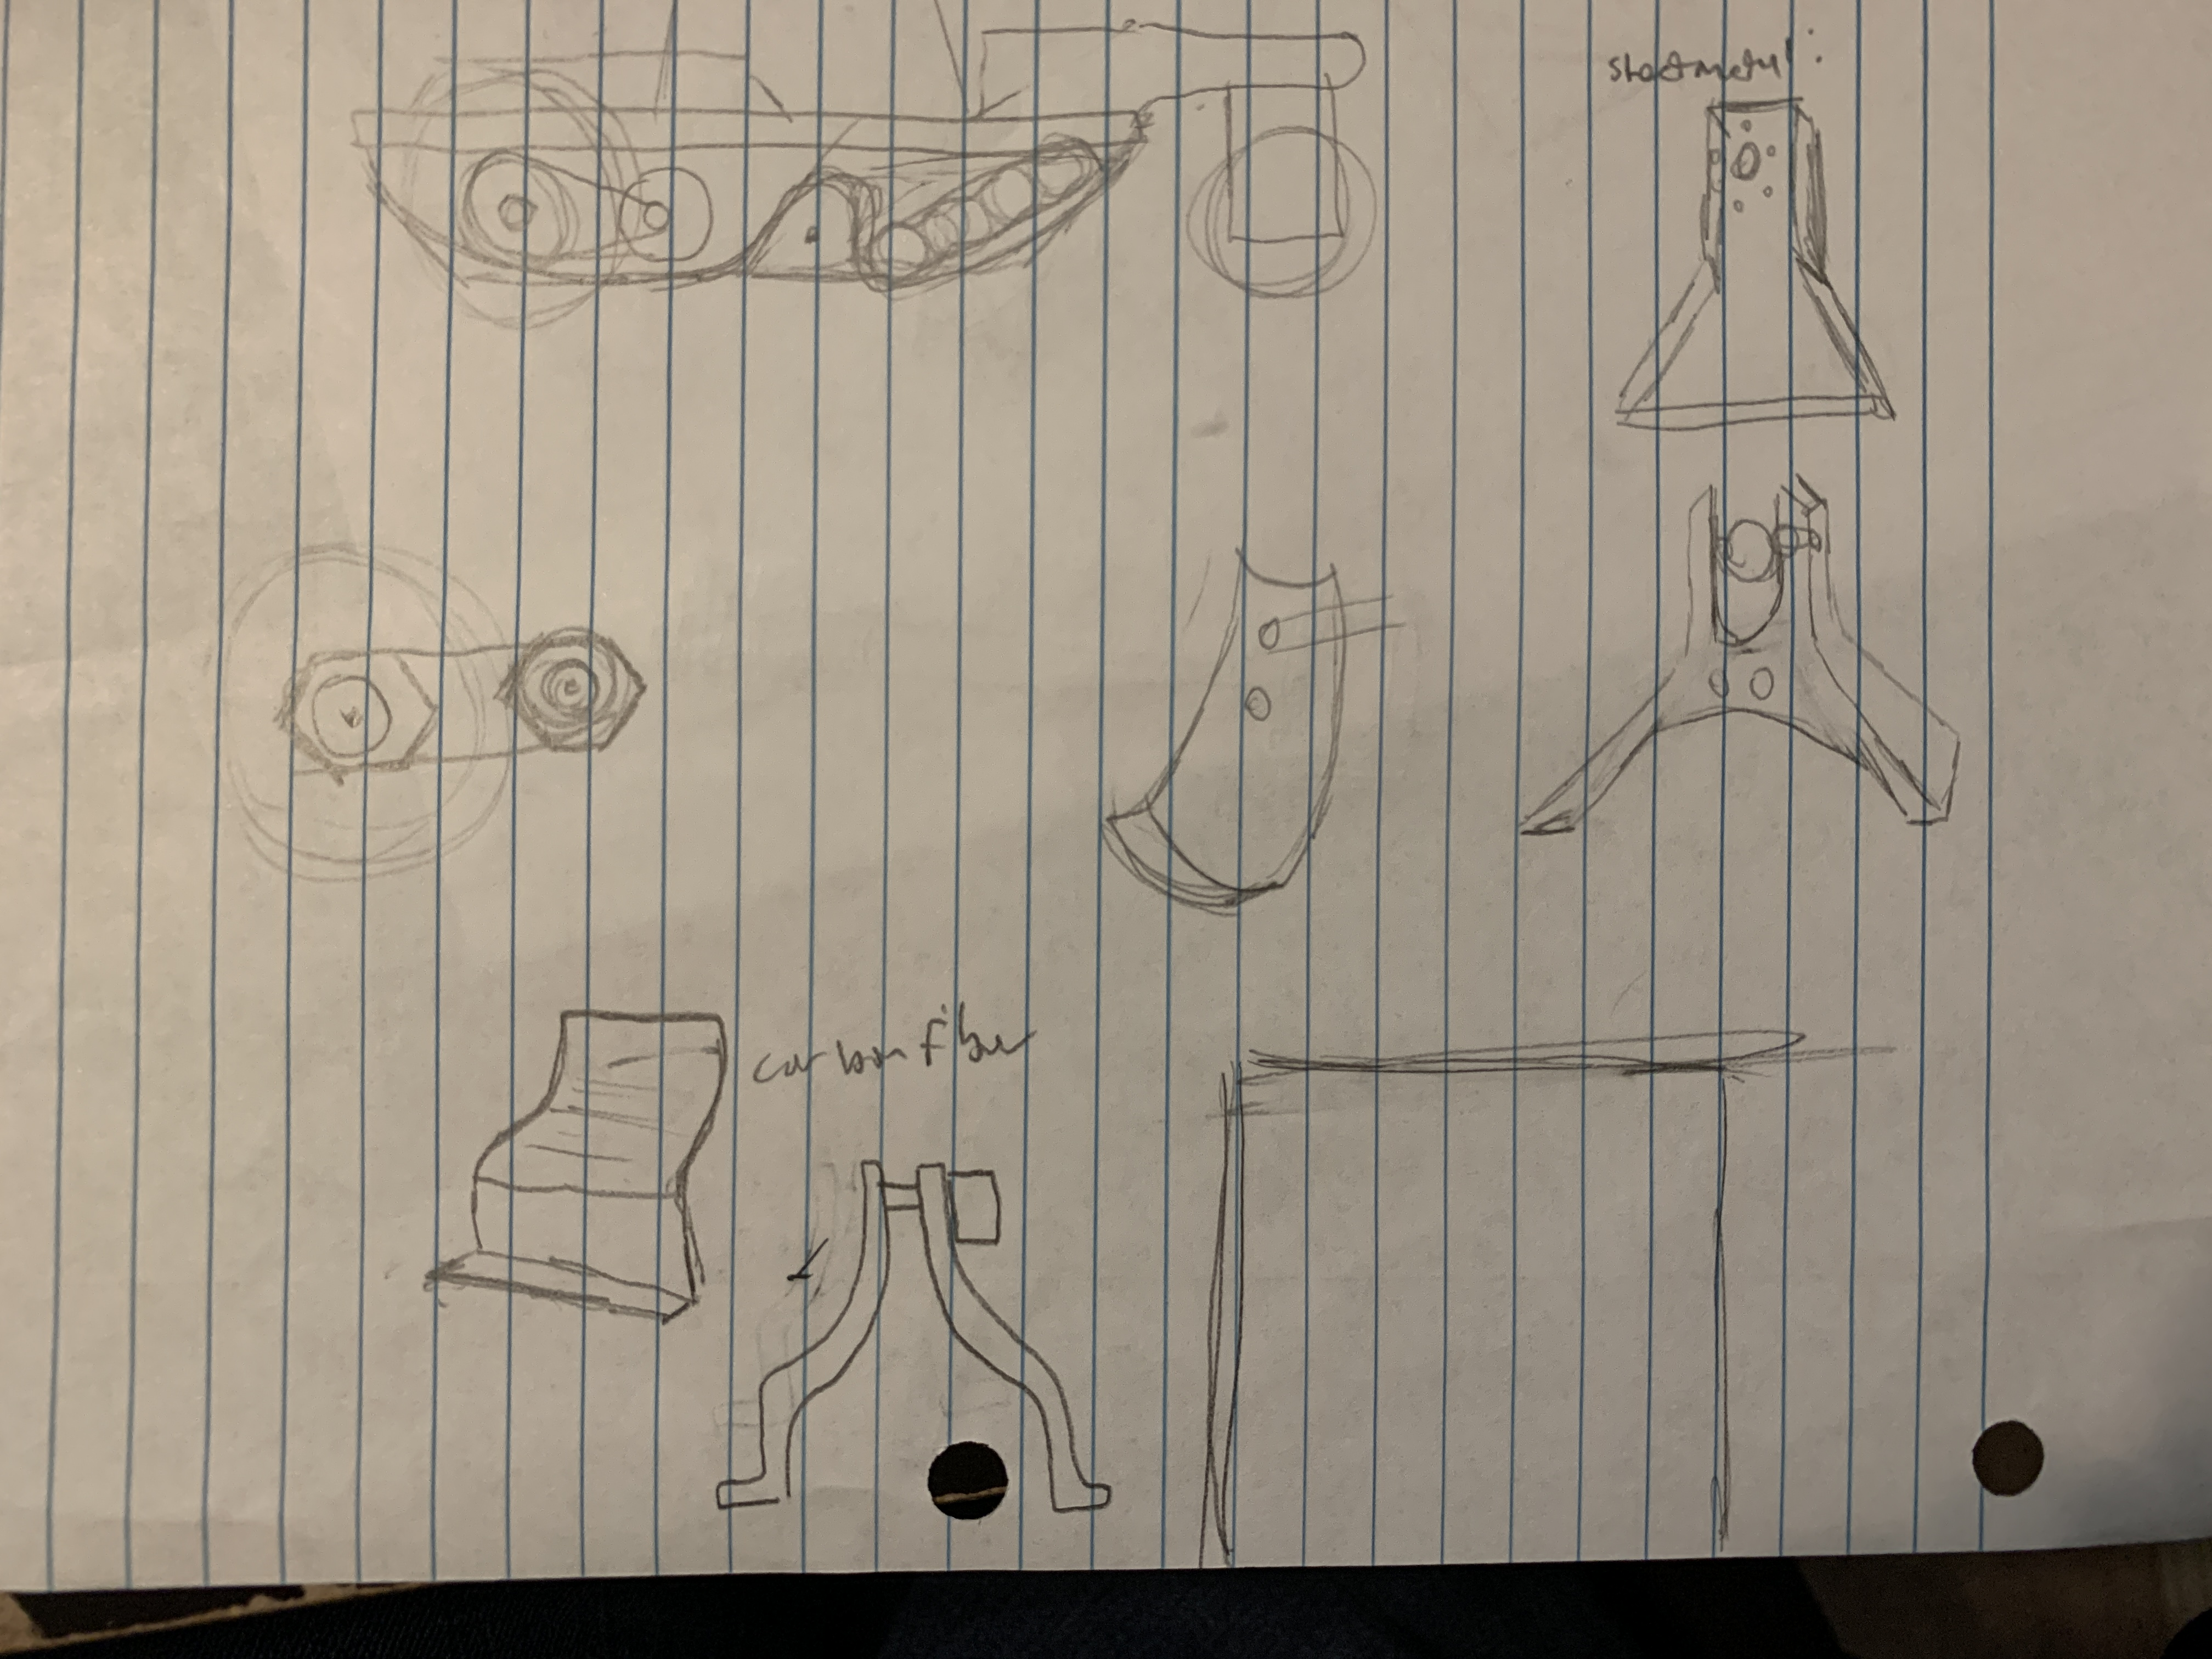
\includegraphics[width=0.95\textwidth]{Meetings/November/11-26-21/11-26-21_CAD_Figure1 - Nathan Forrer.JPG}
  \caption{Sketches of sideplate designs}
  \label{fig:pic1}
\end{minipage}%
\hfill%
\begin{minipage}[b]{.48\textwidth}
  \centering
  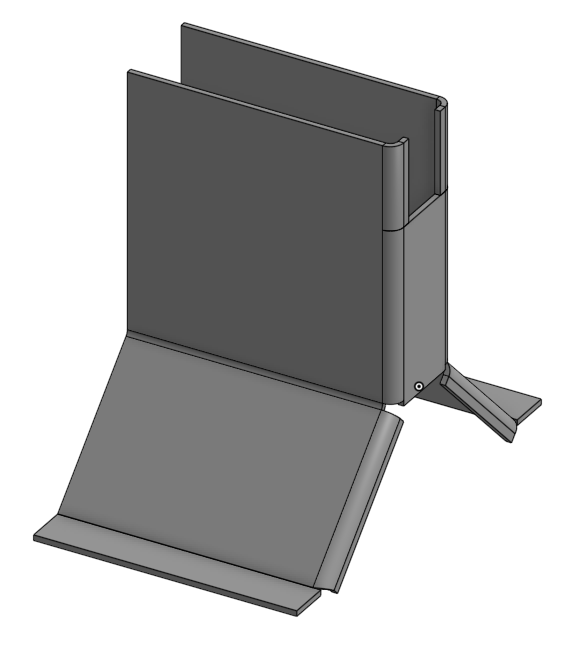
\includegraphics[width=0.95\textwidth]{Meetings/November/11-26-21/11-26-21_CAD_Figure2 - Nathan Forrer.PNG}
  \caption{Sideplate prototypes}
  \label{fig:pic2}
\end{minipage}
\end{figure}

\begin{figure}[ht]
\centering
\begin{minipage}[b]{.48\textwidth}
  \centering
  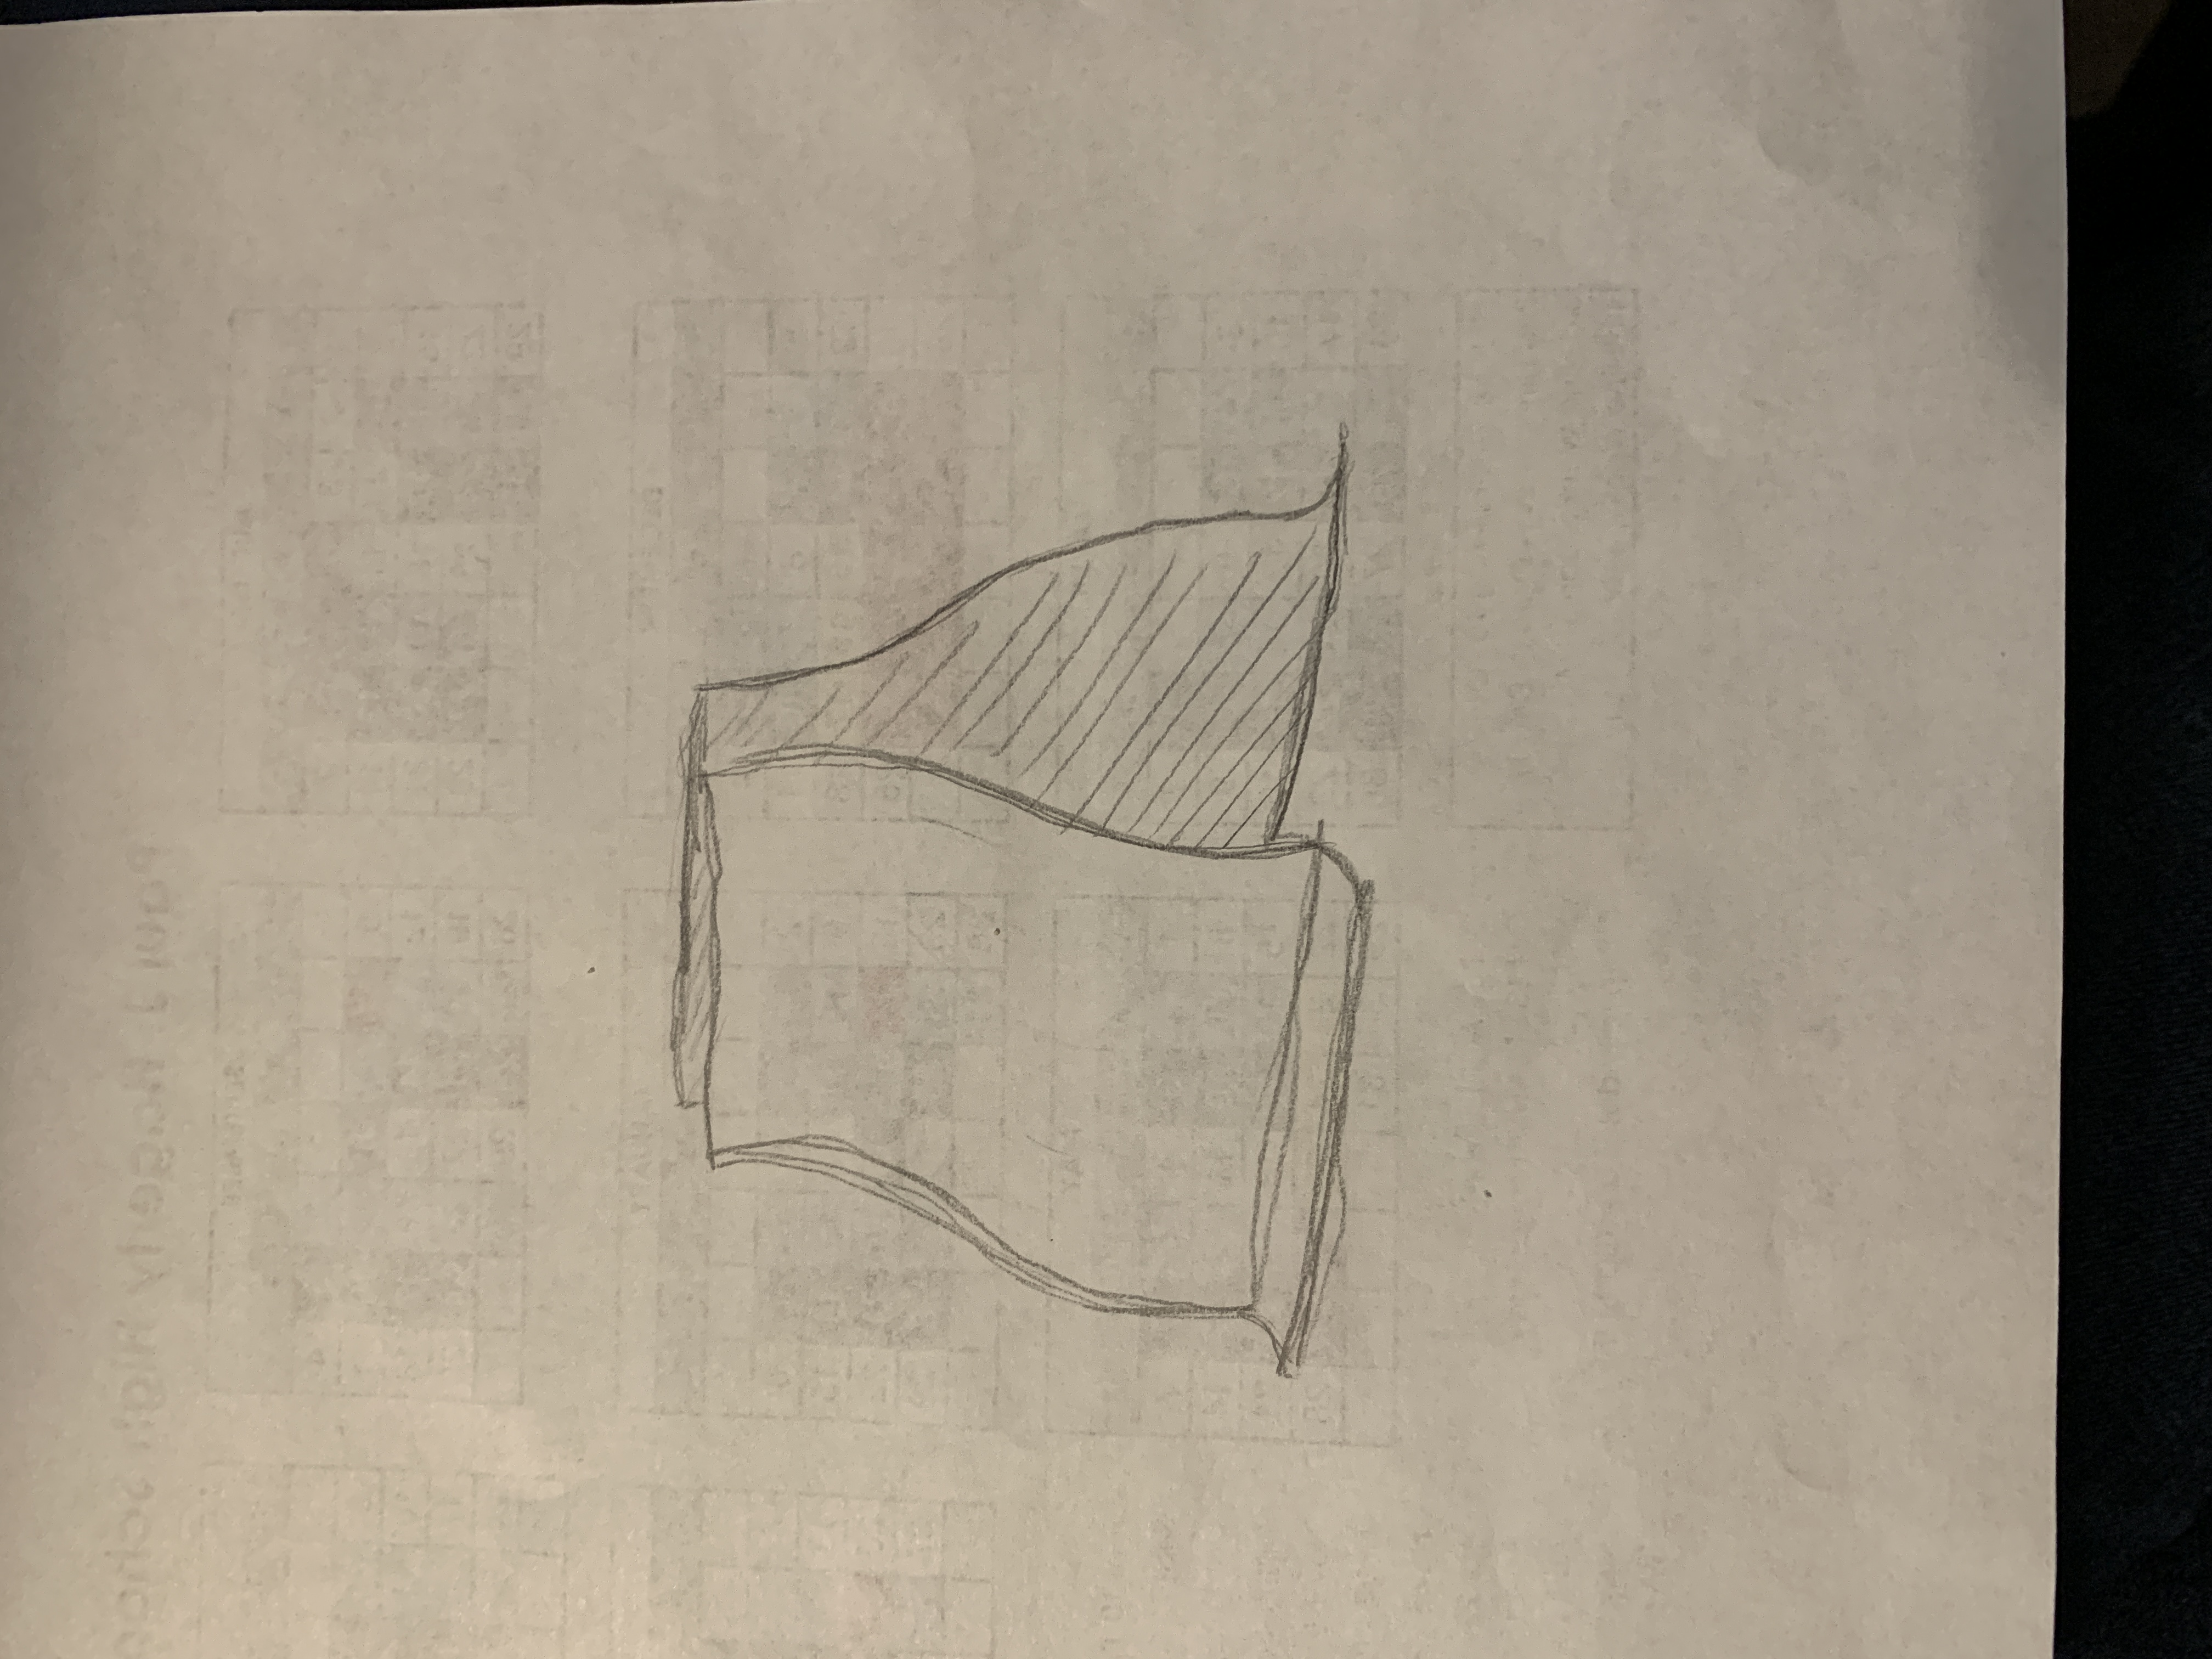
\includegraphics[width=0.95\textwidth]{Meetings/November/11-26-21/11-26-21_CAD_Figure3 - Nathan Forrer.JPG}
  \caption{The final shape of our sideplates}
  \label{fig:pic1}
\end{minipage}%
\hfill%
\begin{minipage}[b]{.48\textwidth}
  \centering
  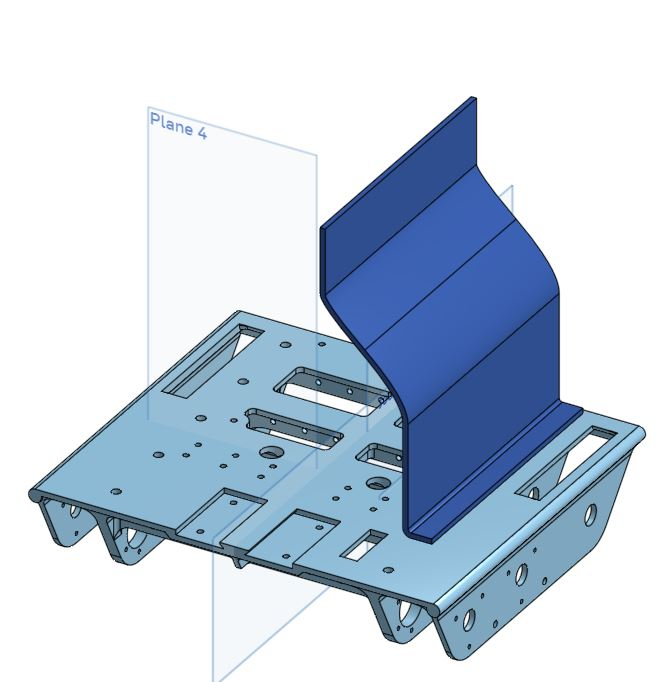
\includegraphics[width=0.95\textwidth]{Meetings/November/11-26-21/11-26-21_CAD_Figure4 - Nathan Forrer.JPG}
  \caption{CAD of the left sideplate}
  \label{fig:pic2}
\end{minipage}
\end{figure}

\begin{figure}[ht]
\centering
\begin{minipage}[b]{.48\textwidth}
  \centering
  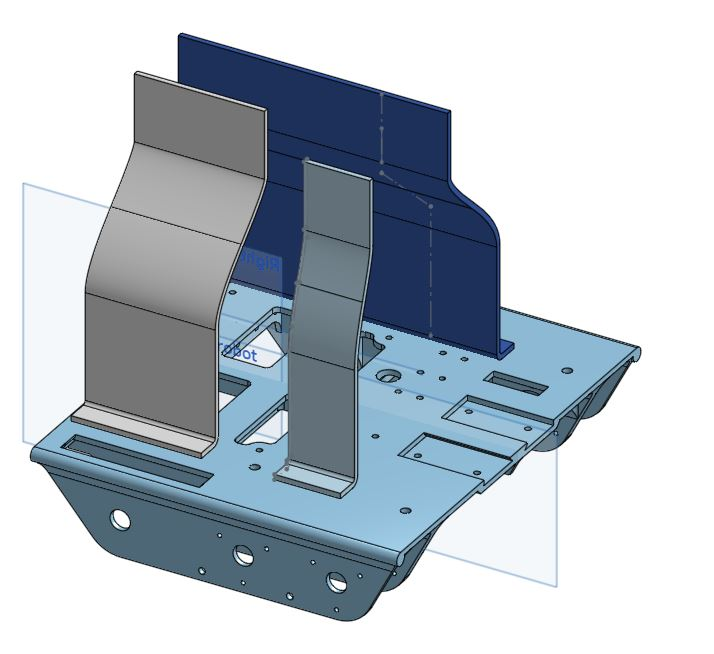
\includegraphics[width=0.95\textwidth]{Meetings/November/11-26-21/11-26-21_CAD_Figure5 - Nathan Forrer.JPG}
  \caption{CAD of the right sideplate with a steeper slope}
  \label{fig:pic1}
\end{minipage}%
\hfill%
\begin{minipage}[b]{.48\textwidth}
  \centering
  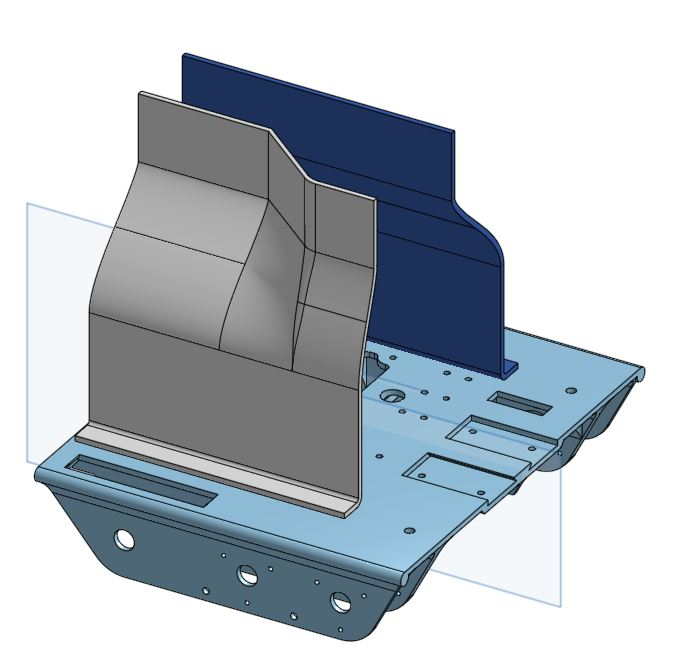
\includegraphics[width=0.95\textwidth]{Meetings/November/11-26-21/11-26-21_CAD_Figure6 - Nathan Forrer.JPG}
  \caption{The completed sideplates}
  \label{fig:pic2}
\end{minipage}
\end{figure}



\whatsnext{
\begin{itemize}
    \item Create molds for carbon fiber sides
    \item Print carbon fiber sides

\end{itemize} 
}

